\documentclass[color={usenames,dvipsnames}]{beamer}

\usetheme{CambridgeUS}

\usepackage{etex}
\reserveinserts{28}

\usepackage{ifthen}

\usepackage[english]{babel}
\usepackage[usenames,dvipsnames]{color}

\usepackage{siunitx}
\usepackage{wasysym}
\usepackage{pgf}
\usepackage{pgfplots}
\usepackage{gnuplot-lua-tikz}
\usepackage{tikz}
\usepackage{pifont}
\usepackage[utf8x]{inputenc}
\usepackage{verbatim}
\usepackage{graphicx}
\usepackage{fontenc}
\usepackage[active]{srcltx}
\usepackage{amsmath}
\usepackage{amsfonts}
\usepackage{amssymb}
\usepackage{amsthm}
\usepackage{graphicx}
\usepackage{url}
\usepackage{prettyref}
\usepackage{epsfig}
\usepackage{fancyhdr}
\usepackage{fancybox}
\usepackage{wasysym}
\usepackage{booktabs}
\usepackage{float}
\usepackage{listings}
\usepackage{amsmath}
\usepackage{psfrag}
\usepackage{pstricks,pst-grad,pst-node,pst-text,pst-3d} 
\usepackage{gensymb}
\usepackage{nicefrac}
\usepackage{xspace}
\usepackage[normalem]{ulem}
\usepackage{placeins}
\usepackage{bm}
\usepackage{bbm}
\usepackage{mathtools}

\definecolor{darkgreen}{rgb}{0,0.7,0}

\newcommand{\good}{\smiley}
\newcommand{\bad}{\frownie}

\setbeamercovered{dynamic}

\mode<article>
{
  \usepackage{fullpage}
  \usepackage{hyperref}
}

\newcommand{\mytitle}{Rating players in large, sparse competitions}

\title{\mytitle}

\author[{E}. {F}onn]{Eivind Fonn}
\institute{SINTEF ICT}
\date{May 21, 2015}

% Approximately equal to

\newcommand{\appropto}{\mathrel{\vcenter{
      \offinterlineskip\halign{\hfil$##$\cr
        \propto\cr\noalign{\kern2pt}\sim\cr\noalign{\kern-2pt}}}}}

% Smiley and frowney items
\newcommand{\startsmitemize}{\vspace{0.15cm}}
\newcommand{\smitem}{\vspace{0.1cm}\noindent\smiley\;}
\newcommand{\fritem}{\vspace{0.1cm}\noindent\frownie\;}

% Number systems, fields, rings, groups...
\newcommand{\bbR}{\mathbb{R}}
\newcommand{\bbC}{\mathbb{C}}
\newcommand{\bbZ}{\mathbb{Z}} 
\newcommand{\bbN}{\mathbb{N}}
\newcommand{\bbS}{\mathbb{S}}

% Calligraphic style
\newcommand{\cA}{\mathcal{A}}
\newcommand{\cB}{\mathcal{B}}
\newcommand{\cD}{\mathcal{D}}
\newcommand{\cE}{\mathcal{E}}
\newcommand{\cF}{\mathcal{F}}
\newcommand{\cI}{\mathcal{I}}
\newcommand{\cL}{\mathcal{L}}
\newcommand{\cM}{\mathcal{M}}
\newcommand{\cN}{\mathcal{N}}
\newcommand{\cO}{\mathcal{O}}
\newcommand{\cP}{\mathcal{P}}
\newcommand{\cS}{\mathcal{S}}
\newcommand{\cT}{\mathcal{T}}

% Roman style
\newcommand{\rmK}{\mathsf{K}}
\newcommand{\rmM}{\mathsf{M}}
\newcommand{\rmP}{\mathsf{P}}
\newcommand{\rmS}{\mathsf{S}}

\newcommand{\rmm}{\mathsf{m}}
\newcommand{\rmp}{\mathsf{p}}
\newcommand{\rms}{\mathsf{s}}

\newcommand{\rmsp}{\mathsf{sp}}

% Boldface
\newcommand{\Ba}{{\bm a}}
\newcommand{\Bb}{{\bm b}}
\newcommand{\Bc}{{\bm c}}
\newcommand{\Bd}{{\bm d}}
\newcommand{\Be}{{\bm e}}
\newcommand{\Bg}{{\bm g}}
\newcommand{\Bk}{{\bm k}}
\newcommand{\Bl}{{\bm \ell}}
\newcommand{\Bm}{{\bm m}}
\newcommand{\Bn}{{\bm n}}
\newcommand{\Bp}{{\bm p}}
\newcommand{\Bq}{{\bm q}}
\newcommand{\Bs}{{\bm s}}
\newcommand{\Bu}{{\bm u}}
\newcommand{\Bv}{{\bm v}}
\newcommand{\Bw}{{\bm w}}
\newcommand{\Bx}{{\bm x}}
\newcommand{\By}{{\bm y}}

\newcommand{\BA}{{\bm A}}

\newcommand{\Bzeta}{{\bm\zeta}}
\newcommand{\Bxi}{{\bm\xi}}
\newcommand{\Bsig}{{\bm\sigma}}
\newcommand{\Bsigma}{\Bsig}
\newcommand{\Balpha}{{\bm\alpha}}
\newcommand{\Bbeta}{{\bm\beta}}

\newcommand{\Bzero}{{\bm0}}

% Symbols
\newcommand{\defeq}{\vcentcolon=}
\newcommand{\eqdef}{=\vcentcolon}

% Hats
\newcommand{\hf}{\hat{f}}
\newcommand{\hbeta}{\hat{\beta}}

\newcommand{\hPsi}{\hat{\Psi}}

% Symbols in special fonts
\newcommand{\blfa}{{\sf a}}
\newcommand{\lfl}{{\ell}}
\newcommand{\ii}{\mathsf{i}}
\newcommand{\ee}{\mathsf{e}}

% Algorithmic
\newcommand{\BREAK}{\STATE \textbf{BREAK}}

\usefont{T1}{cmtt}{m}{n}

% Notes, etc.
\newcommand{\todo}[1]{{\color{red}\textbf{TODO:} #1}}

% Listing
\definecolor{Number}{rgb}{0.0,0.0,1.0}
\definecolor{Keyword}{rgb}{0.8,0.3,0.0}
\definecolor{UDKeyword}{rgb}{0.2,0.7,0.0}
\definecolor{Comment}{rgb}{0.5,0.5,0.5}
\definecolor{String}{rgb}{0.7,0.0,0.6}
\lstloadlanguages{Matlab}
\lstdefinestyle{matlab}{
  language=Matlab
  , frame=single
  % 
  , basicstyle=\scriptsize\ttfamily
  , keywordstyle=[1]\color{Keyword}
  , keywordstyle=[2]\color{UDKeyword}
  , identifierstyle=
  , commentstyle=\color{Comment}
  , stringstyle=\color{String}
  % 
  , numbers=left
  , stepnumber=1
  , numbersep=5pt
  , numberstyle=\tiny\color{Number}\ttfamily
  % 
  , tabsize=4
  , showspaces=false
  , showstringspaces=false
  % 
  , morekeywords={xlim,ylim,varargin,varargout,nargin,nargout,persistent,switch,case,ones,zeros,isfield,mod,
    setdiff,repmat,parfor}
  , deletekeywords={qr}
  , morekeywords=[2]{Settings,GetShearlet,RefreshShearletData,Right,Up,Flip,GetShearletCorners,
    GetTransform,PreparePoints,EvaluateShearlet,EvaluateShearletGradient,BLFKK,BLFSS,BLFSK,
    BLF,LFK,LFS,CheckPolygonIntersection,CheckShearletIntersection,GetIntersection,
    BuildPolygon,PolygonClip,CrossesBoundary,AddToPol,SplitTriangle,BuildQuadRuleOnPolygon,
    TransformQuadRule,BuildSingleQuadRule,IntegrateBLF,IntegrateLF,EvaluateBLF,EvaluateLF,
    BuildDoubleQuadRule,Stiffness,Load}
  , morecomment=[l][\color{Comment}]{...}
}
\lstdefinestyle{c}{
  language=C
  , frame=single
  % 
  , basicstyle=\scriptsize\ttfamily
  , keywordstyle=[1]\color{Keyword}
  , keywordstyle=[2]\color{UDKeyword}
  , identifierstyle=
  , commentstyle=\color{Comment}
  , stringstyle=\color{String}
  % 
  , numbers=left
  , stepnumber=1
  , numbersep=5pt
  , numberstyle=\tiny\color{Number}\ttfamily
  % 
  , tabsize=4
  , showspaces=false
  , showstringspaces=false
  % 
  , morekeywords={pragma}
  , morekeywords=[2]{evaluate_bfun,laguerre_evaluate_zero,laguerre_evaluate_one,q_to_l,l_to_q,
    init_quad_radial,init_quad_angular,init_quad,inner,full_inner,outer,full_outer,
    tensor_index,add_loss,compute,init_jobs_queue,collide,vector_index,rk_timestep,
    adapt_check,init_jobs_alloc,free_jobs_alloc,free_jobs_queue}
  , morecomment=[l][\color{Comment}]{...}
}

% Operators
\DeclareMathOperator{\lcm}{lcm}
\DeclareMathOperator{\supp}{supp}
\DeclareMathOperator{\idty}{Id}
\DeclareMathOperator{\spann}{span}
\DeclareMathOperator{\Mod}{mod}

\newcommand{\dd}{\,\text{d}}
\newcommand{\fdd}{\text{d}}

% Shearlet chapter notation
\newcommand{\aPsi}[5]{\Psi_{#1,#2,#3}^{#4,#5}}
\newcommand{\numatlevel}{\operatorname{NumAtLevel}}
\newcommand{\numright}{\operatorname{NumRight}}
\newcommand{\numup}{\operatorname{NumUp}}
\newcommand{\numshears}{\operatorname{NumShears}}
\newcommand{\nummothers}{\operatorname{NumMothers}}
\newcommand{\stepright}{\operatorname{StepRight}}
\newcommand{\stepup}{\operatorname{StepUp}}
\newcommand{\shear}{\operatorname{Shear}}
\newcommand{\basetrf}{\operatorname{BaseTransform}}
\newcommand{\trf}{\operatorname{Transform}}
\newcommand{\corners}{\operatorname{Corners}}
\newcommand{\checkintersection}{\operatorname{CheckIntersection}}
\newcommand{\computeintersection}{\operatorname{ComputeIntersection}}
\newcommand{\splitpolygon}{\operatorname{SplitPolygon}}
\newcommand{\transformquadrule}{\operatorname{TransformQuadrule}}
\newcommand{\builddquadrule}{\operatorname{BuildDoubleQuadrule}}
\newcommand{\buildsquadrule}{\operatorname{BuildSingleQuadrule}}
\newcommand{\evalblf}{\operatorname{EvalBLF}}
\newcommand{\evallf}{\operatorname{EvalLF}}
\newcommand{\preparepoints}{\operatorname{PreparePoints}}
\newcommand{\modd}{\;\operatorname{\textbf{mod}}\;}

% Boltzmann chapter notation
\newcommand{\Bt}{\tilde{B}}
\newcommand{\B}{\mathcal{B}}
\newcommand{\Bsr}{\B_{\sqrt{2}R}}
\newcommand{\Btr}{\B_{2R}}
\newcommand{\AFF}{\cA_\text{FF}}
\newcommand{\ml}{\lambda^{(+)}}
\newcommand{\LtDl}{{L^2(\cD_L)}}
\newcommand{\PA}{{P_\cA}}
\newcommand{\Qt}{Q_\text{lin}}

% Circled characters
\newcommand*\circled[1]{\tikz[baseline=(char.base)]{
    \node[shape=circle,draw,inner sep=2pt] (char) {#1};}}


\begin{document}

\begin{frame}
  \titlepage
\end{frame}

\section{Problem description}

\begin{frame}
  \frametitle{Problem description}
  
  A large population of players compete in tournaments over time.
  \begin{itemize}
    \item Tournaments are not centrally organized.
    \item The ``meeting'' matrix is sparse to rank players by conventional
      means.
  \end{itemize}

  We need a {\em rating system} that assigns to every player a time-dependent
  {\em playing strength} depending on the results and strengths of his opponents.

  \begin{itemize}
    \item Chess (Elo system).
    \item Various e-sports.
    \item Tennis (ATP rankings work differently).
  \end{itemize}
\end{frame}

\section{Probability model}

\begin{frame}
  \frametitle{Probability model}

  Bradley-Terry model: For two objects with merit parameters $\lambda_1$ and
  $\lambda_2$, object $1$ is preferred to object $2$ with probability
  $\nicefrac{\lambda_1}{(\lambda_1+\lambda_2)}$.

  \vspace{0.3cm}

  Let $\theta_i, \theta_j$ be the strenghts of players $i$ and $j$ at some time,
  and let
  \[
    s =
    \begin{cases}
      1, & \text{$i$ won over $j$}, \\
      -1, & \text{$i$ lost to $j$}. \\
    \end{cases}
  \]
  Then we have the model for game outcomes
  \[
    \rmP(s) = \frac{1}{1 + \ee^{s(\theta_j - \theta_i)}} = \Phi_\cL(s\Delta_{ij}),
  \]
  where $\lambda = \ee^{\theta}$, and $\Delta_{ij} = \theta_i - \theta_j$ is the
  difference in playing strengths.
\end{frame}

\section{Distributions}

\begin{frame}
  \frametitle{Significance of the distribution}
  
  The Bradley-Terry model gives a logistic distribution, but in practice we can
  choose anything.
  \[
    P(s) = \Phi(s\Delta_{ij})
  \]

  \begin{center}
    \begin{tikzpicture}[gnuplot, scale=0.5]
%% generated with GNUPLOT 5.0p0 (Lua 5.3; terminal rev. 99, script rev. 100)
%% Thu 21 May 2015 01:43:05 PM CEST
    \draw[thin, lightgray, step=0.3] (0,0) grid (11.7,6.9);
\path (-0.460,-0.368) rectangle (12.240,7.252);
\gpcolor{color=gp lt color border}
\gpsetlinetype{gp lt border}
\gpsetdashtype{gp dt solid}
\gpsetlinewidth{1.00}
\draw[gp path] (0.000,6.883)--(0.000,0.000)--(11.687,0.000)--(11.687,6.883)--cycle;
\gpcolor{rgb color={0.580,0.000,0.827}}
\draw[gp path] (0.000,0.000)--(0.118,0.000)--(0.236,0.000)--(0.354,0.000)--(0.472,0.000)%
  --(0.590,0.000)--(0.708,0.000)--(0.826,0.000)--(0.944,0.000)--(1.062,0.000)--(1.181,0.000)%
  --(1.299,0.000)--(1.417,0.000)--(1.535,0.000)--(1.653,0.000)--(1.771,0.000)--(1.889,0.000)%
  --(2.007,0.000)--(2.125,0.000)--(2.243,0.000)--(2.361,0.000)--(2.479,0.000)--(2.597,0.000)%
  --(2.715,0.001)--(2.833,0.001)--(2.951,0.002)--(3.069,0.003)--(3.187,0.005)--(3.305,0.008)%
  --(3.423,0.013)--(3.542,0.020)--(3.660,0.031)--(3.778,0.046)--(3.896,0.068)--(4.014,0.098)%
  --(4.132,0.139)--(4.250,0.194)--(4.368,0.265)--(4.486,0.358)--(4.604,0.473)--(4.722,0.616)%
  --(4.840,0.789)--(4.958,0.994)--(5.076,1.232)--(5.194,1.503)--(5.312,1.805)--(5.430,2.136)%
  --(5.548,2.491)--(5.666,2.863)--(5.784,3.248)--(5.903,3.635)--(6.021,4.020)--(6.139,4.392)%
  --(6.257,4.747)--(6.375,5.078)--(6.493,5.380)--(6.611,5.651)--(6.729,5.889)--(6.847,6.094)%
  --(6.965,6.267)--(7.083,6.410)--(7.201,6.525)--(7.319,6.618)--(7.437,6.689)--(7.555,6.744)%
  --(7.673,6.785)--(7.791,6.815)--(7.909,6.837)--(8.027,6.852)--(8.145,6.863)--(8.264,6.870)%
  --(8.382,6.875)--(8.500,6.878)--(8.618,6.880)--(8.736,6.881)--(8.854,6.882)--(8.972,6.882)%
  --(9.090,6.883)--(9.208,6.883)--(9.326,6.883)--(9.444,6.883)--(9.562,6.883)--(9.680,6.883)%
  --(9.798,6.883)--(9.916,6.883)--(10.034,6.883)--(10.152,6.883)--(10.270,6.883)--(10.388,6.883)%
  --(10.506,6.883)--(10.625,6.883)--(10.743,6.883)--(10.861,6.883)--(10.979,6.883)--(11.097,6.883)%
  --(11.215,6.883)--(11.333,6.883)--(11.451,6.883)--(11.569,6.883)--(11.687,6.883);
\gpcolor{rgb color={0.000,0.620,0.451}}
\draw[gp path] (0.000,0.006)--(0.118,0.007)--(0.236,0.008)--(0.354,0.010)--(0.472,0.011)%
  --(0.590,0.013)--(0.708,0.015)--(0.826,0.017)--(0.944,0.019)--(1.062,0.022)--(1.181,0.026)%
  --(1.299,0.030)--(1.417,0.034)--(1.535,0.039)--(1.653,0.045)--(1.771,0.052)--(1.889,0.060)%
  --(2.007,0.069)--(2.125,0.079)--(2.243,0.091)--(2.361,0.105)--(2.479,0.120)--(2.597,0.138)%
  --(2.715,0.159)--(2.833,0.182)--(2.951,0.209)--(3.069,0.239)--(3.187,0.274)--(3.305,0.314)%
  --(3.423,0.359)--(3.542,0.411)--(3.660,0.469)--(3.778,0.534)--(3.896,0.608)--(4.014,0.692)%
  --(4.132,0.785)--(4.250,0.888)--(4.368,1.004)--(4.486,1.131)--(4.604,1.271)--(4.722,1.424)%
  --(4.840,1.591)--(4.958,1.770)--(5.076,1.962)--(5.194,2.167)--(5.312,2.382)--(5.430,2.607)%
  --(5.548,2.839)--(5.666,3.078)--(5.784,3.320)--(5.903,3.563)--(6.021,3.805)--(6.139,4.044)%
  --(6.257,4.276)--(6.375,4.501)--(6.493,4.716)--(6.611,4.921)--(6.729,5.113)--(6.847,5.292)%
  --(6.965,5.459)--(7.083,5.612)--(7.201,5.752)--(7.319,5.879)--(7.437,5.995)--(7.555,6.098)%
  --(7.673,6.191)--(7.791,6.275)--(7.909,6.349)--(8.027,6.414)--(8.145,6.472)--(8.264,6.524)%
  --(8.382,6.569)--(8.500,6.609)--(8.618,6.644)--(8.736,6.674)--(8.854,6.701)--(8.972,6.724)%
  --(9.090,6.745)--(9.208,6.763)--(9.326,6.778)--(9.444,6.792)--(9.562,6.804)--(9.680,6.814)%
  --(9.798,6.823)--(9.916,6.831)--(10.034,6.838)--(10.152,6.844)--(10.270,6.849)--(10.388,6.853)%
  --(10.506,6.857)--(10.625,6.861)--(10.743,6.864)--(10.861,6.866)--(10.979,6.868)--(11.097,6.870)%
  --(11.215,6.872)--(11.333,6.873)--(11.451,6.875)--(11.569,6.876)--(11.687,6.877);
\gpcolor{color=gp lt color border}
\draw[gp path] (0.000,6.883)--(0.000,0.000)--(11.687,0.000)--(11.687,6.883)--cycle;
%% coordinates of the plot area
\gpdefrectangularnode{gp plot 1}{\pgfpoint{0.000cm}{0.000cm}}{\pgfpoint{11.687cm}{6.883cm}}
\end{tikzpicture}
%% gnuplot variables

  \end{center} 

  If A beats B $65$\% of the time, and B beats C $65$\% of the time, how often
  does A beat C?  Logistic: $77.5$\%, normal: $78$\%.
\end{frame}

\begin{frame}
  \frametitle{Player skill distributions}

  The playing strength of each player (for any given game) is normally
  distributed, with assumed known mean and variance.
  \[
    \theta_i \,|\, \mu_i, \sigma_i^2 \;\sim\; \cN(\mu_i, \sigma_i^2)
  \]
  We want to find out how to update $\mu_i$ (the rating) and $\sigma_i^2$ (the
  variance) as a function of time and played games.
\end{frame}

\section{Rating updates}

\begin{frame}
  \frametitle{Rating updates}

  When players don't play, their rating variance increases
  \[
    \sigma_i^2(t_0 + t) = \sigma_i^2(t_0) + \nu^2t
  \]
  
  When players \emph{do} play, we use a Bayesian inversion formula to update
  their ratings.  Essentially,
  \begin{itemize}
    \item The performance rating in a given period is the rating at which the
      likelihood of the actual results is maximized.
    \item The new rating is a weighted average of the current rating and the
      performance rating.  The weight depends on the variances.
    \item The new variance is half the harmonic mean of the variances. It is
      always smaller than before.
  \end{itemize}
  None of the above is ``made up''.
\end{frame}

\begin{frame}
  \frametitle{Other considerations}

  \begin{itemize}
  \item Players start with rating $\theta \sim \cN(0,\sigma^2_{\text{init}})$.
  \item Do not allow $\sigma^2$ to leave the range
    $\left(\sigma^2_{\text{min}}, \sigma^2_{\text{max}}\right)$.
  \end{itemize}

  The model must be fitted with parameters 
  $\sigma^2_{\text{init}}, \sigma^2_{\text{min}}, \sigma^2_{\text{max}}, \nu^2$,
  as well as the period length.
  
  In SC2, which is a volatile game, we had to use relatively large values. In
  chess, one might imagine that they would be lower.
\end{frame}

\section{Predictive power}

\begin{frame}
  \frametitle{Predictive power}

  \begin{center}
    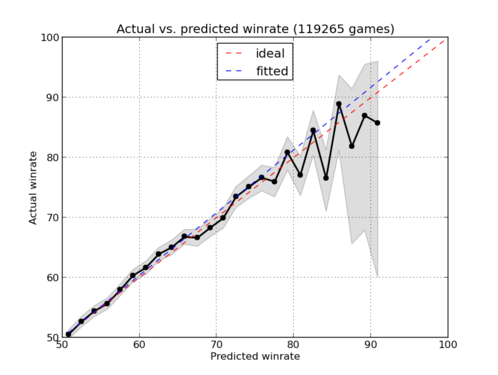
\includegraphics[width=9cm]{figs/predict}
  \end{center}
\end{frame}

\section{Lessons learned}

\begin{frame}
  \frametitle{Lessons learned}

  \begin{itemize}
  \item Proper model fitting is incredibly important. SC2 is a very volatile and fluid game, and it's
    easy to be fooled.
  \item Player pool heterogeneity is a problem. Westerners play with Westerners, Koreans with Koreans,
    etc., but Koreans are generally far stronger.
    \begin{itemize}
    \item Put increased weight on cross-pool matches. (Ineffective.)
    \item Give Koreans bonus starting points. (Crude but effective.)
    \item Clustering algorithms? (Surprisingly ineffective?)
    \end{itemize}
  \end{itemize}
\end{frame}

\section{Today}

\begin{frame}
  \frametitle{Today}

  \begin{itemize}
  \item We have by far the largest and most content-rich SC2 database in the world, and the only one
    that is publicly downloadable and accessible via API.
  \item \num{9300} players, \num{313000} games.
  \item About \num{10000} daily pageviews, enough to hypothetically support hosting costs by a good margin.
  \item About \num{8} currently active teammembers. More than \num{30} have contributed overall,
    \num{8} of those with code.
  \end{itemize}
\end{frame}

\end{document}
